%!TEX root = ../../Compte-rendu.tex
\subsection{Résultats}


\begin{figure}[H]
	\begin{center}
		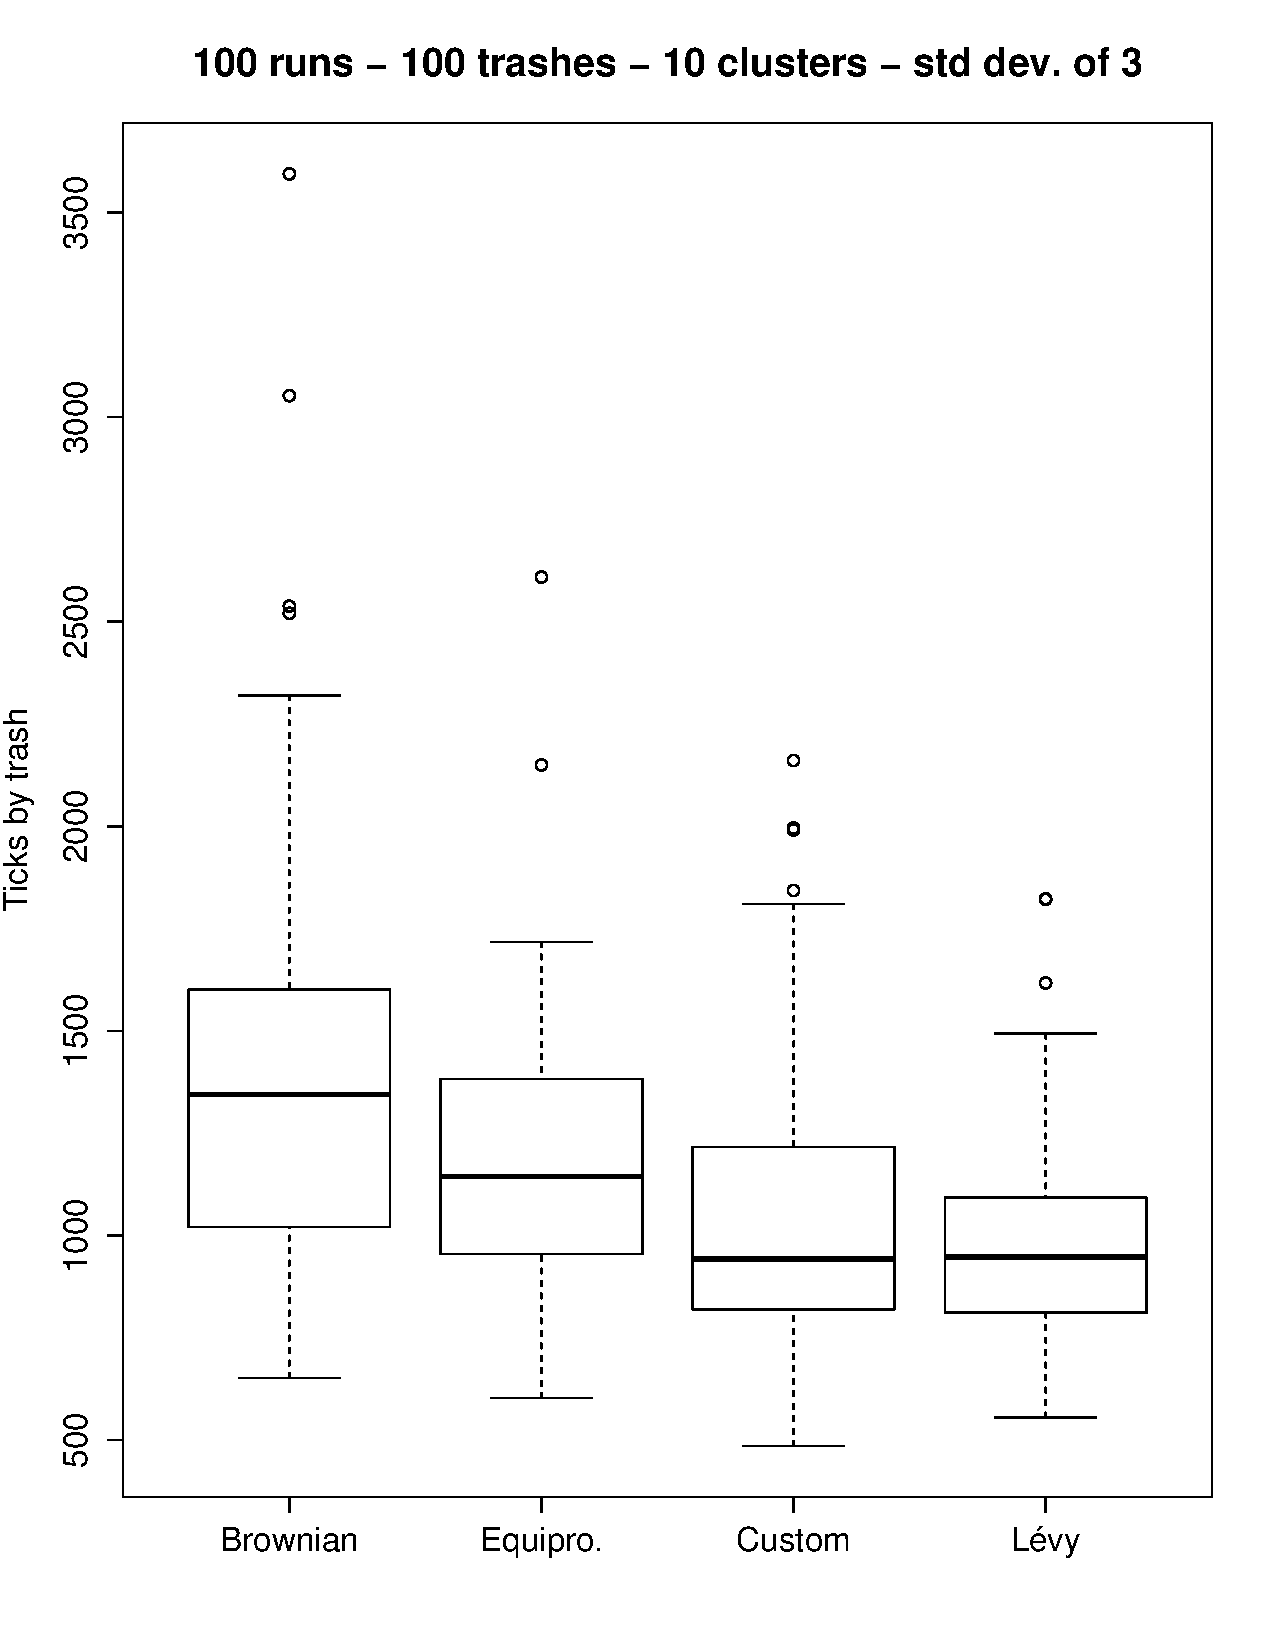
\includegraphics[height=8cm]{diagrams/100Tr10Clts_all.pdf}
		\caption{}
		\label{fig:100Trashes_10Clusters}
	\end{center}
\end{figure}

Nous avons pour les différentes stratégies les médianes suivantes :

\begin{tabular}{ | c | c | }
	\hline
	\multicolumn{2}{ | c | }{Médianes pour la 100 débris distribué en 10 clusters (std dev. = 3)} \\
	\hline
	Brownian & 1344.485 \\
	Equiprobable & 1144.035 \\
	Custom & 942.005 \\
	Lévy & 946.6733 \\
	\hline
\end{tabular}

Nous pouvons constater que la stratégie Custom a une médiane très légèrement meilleure à la stratégie Lévy, néanmoins cette première est moins fiable, c'est à dire qu'elle a plus de chance de produire des résultats bien moins bons que le Lévy.
Nous voyons tout de même que les différent
